
%{{第十五回}}{第十五回}}

\chapter{王熙凤弄权铁槛寺\\秦鲸卿得趣馒头庵}
{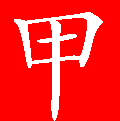
\includegraphics[width=3mm]{../Images/00002}\kaishu 宝玉谒北静王辞对神色,方露出本来面目,迥非在闺阁中之形景。}

{\kaishu 北静王问玉上字果验否,政老对以未曾试过,是隐却多少捕风捉影闲文。}

{\kaishu 北静王论聪明伶俐,又年幼时为溺爱所累,亦大得病源之语。}

{\kaishu 凤姐中火,写纺线村姑,是宝玉闲花野景一得情趣。}

{\kaishu 凤姐另住,明明系秦、玉、智能幽事,却是为净虚钻营凤姐大大一件事作引。}

{\kaishu 秦、智幽情,忽写宝、秦事云:``不知算何账目,未见真切,不曾记得,此系疑案,不敢纂创。''是不落套中,且省却多少累赘笔墨。昔安南国使有题一丈红句云:``五尺墙头遮不得,留将一半与人看。''}

{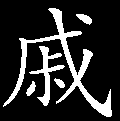
\includegraphics[width=3mm]{../Images/00005}\kaishu 欲显铮铮不避嫌,英雄每入小人缘。鲸卿些子风流事,胆落魂销已可怜。}

诗云:\ldots{}\ldots{}

话说宝玉举目见北静王水溶头上戴着洁白簪缨银翅王帽,穿着江牙海水五爪坐龙白蟒袍,系着碧玉红鞓带,面如美玉,目似明星,真好秀丽人物。宝玉忙抢上来参见,水溶连忙从轿内伸出手来挽住。见宝玉戴着束发银冠,勒着双龙出海抹额,穿着白蟒箭袖,围着攒珠银带,面若春花,目如点漆。{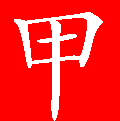
\includegraphics[width=3mm]{../Images/00002}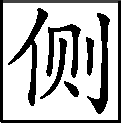
\includegraphics[width=3mm]{../Images/00011}\footnotesize \kaishu 又换此一句,如见其形。}水溶笑道:``名不虚传,果然如`宝'似`玉'。''因问:``衔的那宝贝在那里?''宝玉见问,连忙从衣内取了递与过去。水溶细细的看了,又念了那上头的字,因问:``果灵验否?''贾政忙道:``虽如此说,只是未曾试过。''水溶一面极口称奇道异,一面理好彩绦,亲自与宝玉戴上,{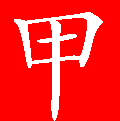
\includegraphics[width=3mm]{../Images/00002}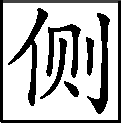
\includegraphics[width=3mm]{../Images/00011}\footnotesize \kaishu 钟爱之至。}又携手问宝玉几岁,读何书。宝玉一一答应。

水溶见他言语清楚,谈吐有致,{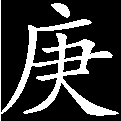
\includegraphics[width=3mm]{../Images/00004}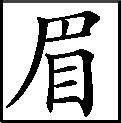
\includegraphics[width=3mm]{../Images/00010}\footnotesize \kaishu 八字道尽玉兄,如此等方是玉兄正文写照。壬午季春。}一面又向贾政笑道:``令郎真乃龙驹凤雏,非小王在世翁前唐突,将来`雏凤清于老凤声',{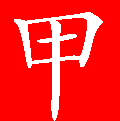
\includegraphics[width=3mm]{../Images/00002}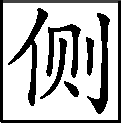
\includegraphics[width=3mm]{../Images/00011}\footnotesize \kaishu 妙极!开口便是西昆体,宝玉闻之,宁不刮目哉?}未可量也。''贾政忙陪笑道:``犬子岂敢谬承金奖。赖藩郡馀祯,果如是言,亦荫生辈之幸矣。''{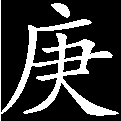
\includegraphics[width=3mm]{../Images/00004}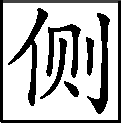
\includegraphics[width=3mm]{../Images/00011}\footnotesize \kaishu 谦的得体。}水溶又道:``只是一件,令郎如是资质,想老太夫人、夫人辈自然钟爱极矣;但吾辈后生,甚不宜钟溺,钟溺则未免荒失学业。昔小王曾蹈此辙,想令郎亦未必不如是也。若令郎在家难以用功,不妨常到寒第。小王虽不才,却多蒙海上众名士凡至都者,未有不另垂青目,是以寒第高人颇聚。令郎常去谈会谈会,则学问可以日进矣。''贾政忙躬身答应。

水溶又将腕上一串念珠卸了下来,递与宝玉道:``今日初会,仓促竟无敬贺之物,此系前日圣上亲赐鹡鸰香\href{../Text/part0019_split_000.html\#lnkback_1_a}{\textsuperscript{①}}念珠一串,权为贺敬之礼。''宝玉连忙接了,回身奉与贾政。{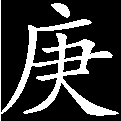
\includegraphics[width=3mm]{../Images/00004}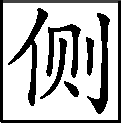
\includegraphics[width=3mm]{../Images/00011}\footnotesize \kaishu 转出没调教。}贾政与宝玉一齐谢过。于是贾赦、贾珍等一齐上来请回舆,水溶道:``逝者已登仙界,非碌碌你我尘寰中之人也。小王虽上叩天恩,虚邀郡袭,岂可越仙輀而进也?''贾赦等见执意不从,只得告辞谢恩回来,命手下掩乐停音,滔滔然将殡过完,{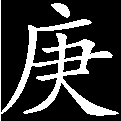
\includegraphics[width=3mm]{../Images/00004}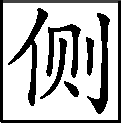
\includegraphics[width=3mm]{../Images/00011}\footnotesize \kaishu 有层次,好看煞。}方让水溶回舆去了。不在话下。

且说宁府送殡,一路热闹非常。刚至城门前,又有贾赦、贾政、贾珍等诸同僚属下各家祭棚接祭,一一的谢过,然后出城,竟奔铁槛寺大路行来。彼时贾珍带贾蓉来到诸长辈前,让坐轿上马,因而贾赦一辈的各自上了车轿,贾珍一辈的也将要上马。凤姐因记挂着宝玉,{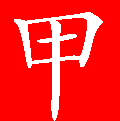
\includegraphics[width=3mm]{../Images/00002}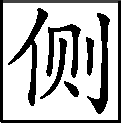
\includegraphics[width=3mm]{../Images/00011}\footnotesize \kaishu 千百件忙事内不漏一丝。 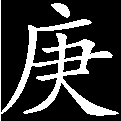
\includegraphics[width=3mm]{../Images/00004}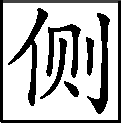
\includegraphics[width=3mm]{../Images/00011}\footnotesize \kaishu 细心人自应如是。}怕他在郊外纵性逞强,不服家人的话,贾政管不着这些小事,惟恐有个闪失,难见贾母,因此便命小厮来唤他。宝玉只得来到他的车前。凤姐笑道:``好兄弟,你是个尊贵人,女孩儿一样的人品,{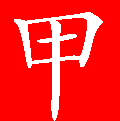
\includegraphics[width=3mm]{../Images/00002}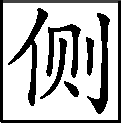
\includegraphics[width=3mm]{../Images/00011}\footnotesize \kaishu 非此一句宝玉必不依,阿凤真好才情。}别学他们猴在马上。下来,咱们姐儿两个坐车,岂不好?''宝玉听说,便忙下了马,爬入凤姐车上,二人说笑前进。

不一时,只见从那边两骑马压地飞来,{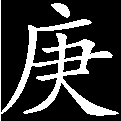
\includegraphics[width=3mm]{../Images/00004}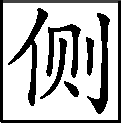
\includegraphics[width=3mm]{../Images/00011}\footnotesize \kaishu 有气有声,有形有影。}离凤姐车不远,一齐蹿下来,扶车回说:``这里有下处,奶奶请歇息、更衣。''凤姐急命请邢夫人、王夫人的示下,{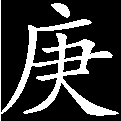
\includegraphics[width=3mm]{../Images/00004}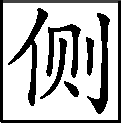
\includegraphics[width=3mm]{../Images/00011}\footnotesize \kaishu 有次序。}那人回来说:``太太们说不用歇了,叫奶奶自便罢。''凤姐听了,便命歇歇再走。众小厮听了,一带辕马,岔出人群,往北飞走。宝玉在车内急命请秦相公。那时秦钟正骑马随着他父亲的轿,忽见宝玉的小厮跑来,请他去打尖。秦钟看时,只见凤姐儿的车往北而去,后面拉着宝玉的马,搭着鞍笼,便知宝玉同凤姐坐车,自己也便带马赶上来,同入一庄门内。早有家人将众庄汉撵尽。那村庄人家无多房舍,婆娘们无处回避,只得由他们去了。那些村姑、庄妇见了凤姐、宝玉、秦钟的人品衣服、礼数款段,岂有不爱看的?

一时凤姐进入茅堂,因命宝玉等先出去顽顽。宝玉等会意,因同秦钟出来,带着小厮们各处游顽。凡庄农动用之物,皆不曾见过。{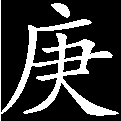
\includegraphics[width=3mm]{../Images/00004}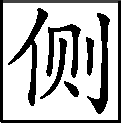
\includegraphics[width=3mm]{../Images/00011}\footnotesize \kaishu 真,毕真!}宝玉一见了锹、锄、镢、犁等物,皆以为奇,不知何项所使,其名为何。{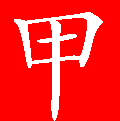
\includegraphics[width=3mm]{../Images/00002}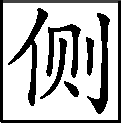
\includegraphics[width=3mm]{../Images/00011}\footnotesize \kaishu 凡膏粱子弟齐来着眼。}小厮在旁一一的告诉了名色,说明原委。{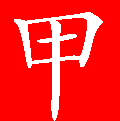
\includegraphics[width=3mm]{../Images/00002}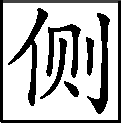
\includegraphics[width=3mm]{../Images/00011}\footnotesize \kaishu 也盖因未见之故也。}宝玉听了,因点头叹道:``怪道古人诗上说:`谁知盘中餐,粒粒皆辛苦',正为此也。''{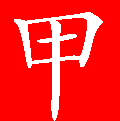
\includegraphics[width=3mm]{../Images/00002}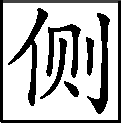
\includegraphics[width=3mm]{../Images/00011}\footnotesize \kaishu 聪明人自是一喝即悟。 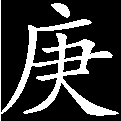
\includegraphics[width=3mm]{../Images/00004}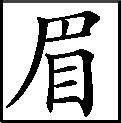
\includegraphics[width=3mm]{../Images/00010}\footnotesize \kaishu 写玉兄正文总于此等处,作者良苦。壬午季春。}一面说,一面又至一间房前,只见炕上有个纺车,宝玉又问小厮们:``这又是什么?''小厮们又告诉他原委。宝玉听说,便上来拧转作耍,自为有趣。只见一个约有十七八岁的村庄丫头跑了来乱嚷:``别动坏了!''{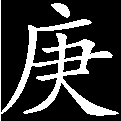
\includegraphics[width=3mm]{../Images/00004}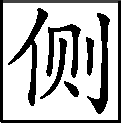
\includegraphics[width=3mm]{../Images/00011}\footnotesize \kaishu 天生地设之文。}众小厮忙断喝拦阻,宝玉忙丢开手,陪笑说道:{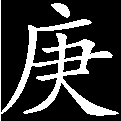
\includegraphics[width=3mm]{../Images/00004}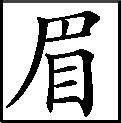
\includegraphics[width=3mm]{../Images/00010}\footnotesize \kaishu 一``忙''字,二``陪笑''字,写玉兄是在女儿分上。壬午季春。}``我因为没见过这个,所以试他一试。''那丫头道:``你们那里会弄这个,站开了,{{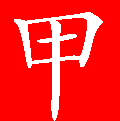
\includegraphics[width=3mm]{../Images/00002}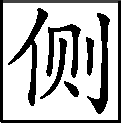
\includegraphics[width=3mm]{../Images/00011}\footnotesize \kaishu 如闻其声,见其形。 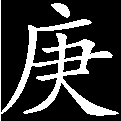
\includegraphics[width=3mm]{../Images/00004}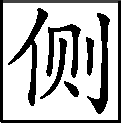
\includegraphics[width=3mm]{../Images/00011}\footnotesize \kaishu 三字如闻。 }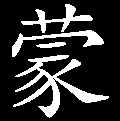
\includegraphics[width=3mm]{../Images/00006}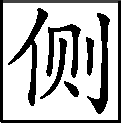
\includegraphics[width=3mm]{../Images/00011}\footnotesize \kaishu 这丫头是技痒,是多情,是自己生活恐至损坏?宝玉此时一片心神,另有主张。}我纺与你瞧。''秦钟暗拉宝玉笑道:``此卿大有意趣。''{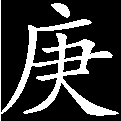
\includegraphics[width=3mm]{../Images/00004}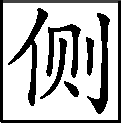
\includegraphics[width=3mm]{../Images/00011}\footnotesize \kaishu 忙中闲笔,却伏下文。}宝玉一把推开,笑道:``该死的!{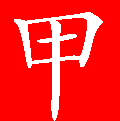
\includegraphics[width=3mm]{../Images/00002}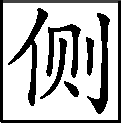
\includegraphics[width=3mm]{../Images/00011}\footnotesize \kaishu 的是宝玉生性之言。}再胡说,我就打了!''{\includegraphics[width=3mm]{../Images/00004}\includegraphics[width=3mm]{../Images/00011}\footnotesize \kaishu 玉兄身分,本心如此。}说着,只见那丫头纺起线来。宝玉正要说话时,{\includegraphics[width=3mm]{../Images/00004}\includegraphics[width=3mm]{../Images/00010}\footnotesize \kaishu 若说话,便不是《石头记》中文字也。}只听那边老婆子叫道:``二丫头,快过来!''那丫头听见,丢下纺车,一径去了。

宝玉怅然无趣。{\includegraphics[width=3mm]{../Images/00002}\includegraphics[width=3mm]{../Images/00011}\footnotesize \kaishu 处处点``情'',又伏下一段后文。}只见凤姐打发人来叫他两个进去。凤姐洗了手,换衣服,抖灰土,问他们换不换。宝玉不换,只得罢了。家下仆妇们将带着行路的茶壶茶杯、十锦屉盒、各样小食端来,凤姐等吃过茶,待他们收拾完备,便起身上车。外面旺儿预备下赏封,赏了本村主人,庄妇等来叩赏。凤姐并不在意,宝玉却留心看时,内中并无二丫头。{\includegraphics[width=3mm]{../Images/00004}\includegraphics[width=3mm]{../Images/00011}\footnotesize \kaishu 妙在不见。}一时上了车,出来走不多远,只见迎头二丫头怀里抱着他小兄弟,{\includegraphics[width=3mm]{../Images/00004}\includegraphics[width=3mm]{../Images/00011}\footnotesize \kaishu 妙在此时方见,错综之妙如此!}同着几个小女孩子说笑而来。宝玉恨不得下车跟了他去,料是众人不依的,少不得以目相送,争奈车轻马快,{\includegraphics[width=3mm]{../Images/00002}\includegraphics[width=3mm]{../Images/00011}\footnotesize \kaishu 四字有文章。人生离聚亦未尝不如此也。}一时展眼无踪。

走不多时,仍又跟上了大殡。早有前面法鼓金铙,幢幡宝盖,铁槛寺接灵众僧齐至。少时,到入寺中,另演佛事,重设香坛。安灵于内殿偏室之中,宝珠安理寝室相伴。外面贾珍款待一应亲友,也有扰饭的,也有不吃饭而辞的,一应谢过乏,从公侯伯子男一起一起的散去,至未末时分方才散尽了。里面的堂客,皆是凤姐张罗接待,先从显官诰命散起,也到晌午大错时方散尽了。只有几个亲戚是至近的,等做过三日安灵道场方去。那时邢、王二夫人知凤姐必不能回家,也便就要进城。王夫人要带宝玉去,宝玉乍到郊外,那里肯回去,只要跟凤姐住着。王夫人无法,只得交与凤姐便回来了。

原来这铁槛寺原是宁荣二公当日修造,现今还是有香火地亩布施,以备京中老了人口,在此便宜寄放。其中阴阳两宅俱已预备妥贴,{\includegraphics[width=3mm]{../Images/00002}\includegraphics[width=3mm]{../Images/00012}\footnotesize \kaishu 大凡创业之人,无有不为子孙深谋至细。奈后辈仗一时之荣显,犹自不足,另生枝叶,虽华丽过先,奈不常保,亦足可叹,争及先人之常保其朴哉!近世浮华子弟齐来着眼。}好为送灵人口寄居。{\includegraphics[width=3mm]{../Images/00002}\includegraphics[width=3mm]{../Images/00011}\footnotesize \kaishu 祖宗为子孙之心细到如此! \includegraphics[width=3mm]{../Images/00004}\includegraphics[width=3mm]{../Images/00010}\footnotesize \kaishu 《石头记》总于没要紧处,闲闲一二笔,写正文筋骨。看官当用巨眼,不为彼瞒过方好。壬午季春。}不想如今后辈人口繁盛,其中贫富不一,或性情参商,{\includegraphics[width=3mm]{../Images/00002}\includegraphics[width=3mm]{../Images/00012}\footnotesize \kaishu 所谓``源远水则浊,枝繁果则稀''。余为天下痴心祖宗为子孙谋千年业者痛哭。}有那家业艰难安分的,{\includegraphics[width=3mm]{../Images/00002}\includegraphics[width=3mm]{../Images/00011}\footnotesize \kaishu 妙在艰难就安分,富贵则不安分矣。}便住在这里了;有那尚排场有钱势的,只说这里不方便,一定另外或村庄或尼庵寻个下处,为事毕宴退之所。{\includegraphics[width=3mm]{../Images/00002}\includegraphics[width=3mm]{../Images/00011}\footnotesize \kaishu 真真辜负祖宗体贴子孙之心。}即今秦氏之丧,族中诸人皆权在铁槛寺下榻,独有凤姐嫌不方便,{\includegraphics[width=3mm]{../Images/00002}\includegraphics[width=3mm]{../Images/00011}\footnotesize \kaishu 不用说,阿凤自然不肯将就一刻的。}因而早遣人来和馒头庵的姑子净虚说了,腾出两间房子来作下处。

原来这馒头庵就是水月寺,因他庙里做的馒头好,就起了这个浑号,离铁槛寺不远。{\includegraphics[width=3mm]{../Images/00002}\includegraphics[width=3mm]{../Images/00012}\footnotesize \kaishu 前人诗云:``纵有千年铁门限,终须一个土馒头。''是此意。故``不远''二字有文章。}当下和尚工课已完,奠过晚茶,贾珍便命贾蓉请凤姐歇息。凤姐见还有几个妯娌陪着女亲,自己便辞了众人,带了宝玉、秦钟往水月庵来。原来秦业年迈多病,{\includegraphics[width=3mm]{../Images/00002}\includegraphics[width=3mm]{../Images/00011}\footnotesize \kaishu 伏一笔。}不能在此,只命秦钟等待安灵罢了。那秦钟便只跟着凤姐、宝玉,一时到了水月庵,净虚带领智善、智能两个徒弟出来迎接,大家见过。凤姐等来至净室更衣净手毕,因见智能儿越发长高了,模样儿越发出息了,因说道:``你们师徒怎么这些日子也不往我们那里去?''净虚道:``可是,这几天都没工夫,因胡老爷府里产了公子,太太送了十两银子来这里,叫请几位师父念三日《血盆经》,忙的无个空儿,就无来请奶奶的安。''{\includegraphics[width=3mm]{../Images/00002}\includegraphics[width=3mm]{../Images/00011}\footnotesize \kaishu 虚陪一个胡姓,妙!言是糊涂人之所为也。}

不言老尼陪着凤姐。且说秦钟、宝玉二人正在殿上顽耍,因见智能过来,宝玉笑道:``能儿来了。''秦钟道:``理那个东西作什么?''宝玉笑道:``你别弄鬼,那一日在老太太屋里,一个人没有,你搂着他作什么?这会子还哄我。''{\includegraphics[width=3mm]{../Images/00002}\includegraphics[width=3mm]{../Images/00011}\footnotesize \kaishu 补出前文未到处,细思秦钟近日在荣府所为,可知矣。}秦钟笑道:``这可是没有的话。''宝玉笑道:``有没有也不管你,你只叫住他倒碗茶来我吃,就丢开手。''秦钟笑道:``这又奇了,你叫他倒去,还怕他不倒?何必要我说呢。''宝玉道:``我叫他倒的是无情意的,不及你叫他倒的是有情意的。''{\includegraphics[width=3mm]{../Images/00002}\includegraphics[width=3mm]{../Images/00011}\footnotesize \kaishu 总作如是等奇语。}秦钟只得说道:``能儿,倒碗茶来给我。''那智能儿自幼在荣府走动,无人不识,因常与宝玉、秦钟顽笑。他如今大了,渐知风月,便看上了秦钟人物风流,那秦钟也极爱他妍媚,二人虽未上手,却已情投意合了。{\includegraphics[width=3mm]{../Images/00002}\includegraphics[width=3mm]{../Images/00011}\footnotesize \kaishu 不爱宝玉,却爱秦钟,亦是各有情孽。}今智能见了秦钟,心眼俱开,走去倒了茶来。秦钟笑说:``给我。''{\includegraphics[width=3mm]{../Images/00002}\includegraphics[width=3mm]{../Images/00011}\footnotesize \kaishu 如闻其声。}宝玉叫:``给我!''智能儿抿嘴笑道:``一碗茶也来争,我难道手里有蜜!''{\includegraphics[width=3mm]{../Images/00002}\includegraphics[width=3mm]{../Images/00011}\footnotesize \kaishu 一语毕肖,如闻其语,观者已自酥倒,不知作者从何着想。}宝玉先抢得了,吃着,方要问话,只见智善来叫智能去摆茶碟子,一时来请他两个去吃茶果点心。他两个那里吃这些东西?坐一坐仍出来顽耍。

凤姐也略坐片时,便回至净室歇息,老尼相送。此时众婆娘媳妇见无事,皆陆续散了,自去歇息,跟前不过几个心腹常侍小婢,老尼便趁机说道:``我正有一事,要到府里求太太,先请奶奶一个示下。''凤姐因问何事。老尼道:``阿弥陀佛!{\includegraphics[width=3mm]{../Images/00002}\includegraphics[width=3mm]{../Images/00011}\footnotesize \kaishu 开口称佛,毕肖。可叹可笑!}只因当日我先在长安县内善才庵{\includegraphics[width=3mm]{../Images/00002}\includegraphics[width=3mm]{../Images/00011}\footnotesize \kaishu ``才''字妙。}内出家的时节,那时有个施主姓张,是大财主。他有个女儿小名金哥,{\includegraphics[width=3mm]{../Images/00002}\includegraphics[width=3mm]{../Images/00011}\footnotesize \kaishu 俱从``财''一字上发生。}那年都往我庙里来进香,不想遇见了长安府府太爷的小舅子李衙内。那李衙内一心看上,要娶金哥,打发人来求亲,不想金哥已受了原任守备的公子的聘礼。张家若退亲,又怕守备不依,因此说有了人家。谁知李公子执意不依,定要娶他女儿。张家正无计策,两处为难。不想守备家听了此信,也不管青红皂白,便来作践辱骂,说一个女儿许几家,偏不许退定礼,就要打官司告状起来。{{\includegraphics[width=3mm]{../Images/00002}\includegraphics[width=3mm]{../Images/00012}\footnotesize \kaishu 守备一闻便{(问)}{[}闹{]}}}\href{../Text/part0019_split_000.html\#lnkback_2_a}{\textsuperscript{②}}{,断无此理。此不过张家惧府尹之势,必先退定礼,守备方不从,或有之。此时老尼只欲与张家完事,故将此言遮饰,以便退亲,受张家之贿也。}那张家急了,{\includegraphics[width=3mm]{../Images/00002}\includegraphics[width=3mm]{../Images/00012}\footnotesize \kaishu 如何便急了,话无头绪,可知张家理缺。此系作者巧摹老尼无头绪之语,莫认作者无头绪,正是神处奇处。摹一人,一人必到纸上活现。}只得着人上京来寻门路,赌气偏要退定礼。{\includegraphics[width=3mm]{../Images/00002}\includegraphics[width=3mm]{../Images/00011}\footnotesize \kaishu 如何?的是张家要与府尹攀亲!}我想如今长安节度云老爷与府上最契,可以求太太与老爷说声,打发一封书去,求云老爷和那守备说一声,不怕那守备不依。若是肯行,张家连倾家孝敬,也都情愿。''{\includegraphics[width=3mm]{../Images/00002}\includegraphics[width=3mm]{../Images/00012}\footnotesize \kaishu 坏极,妙极!若与府尹攀了亲,何惜张财不能再得?小人之心如此,良民遭害如此!}

凤姐听了笑道:``这事倒不大,{\includegraphics[width=3mm]{../Images/00002}\includegraphics[width=3mm]{../Images/00011}\footnotesize \kaishu 五字是阿凤心迹。}只是太太再不管这样的事。''老尼道:``太太不管,奶奶也可以主张了。''凤姐听说笑道:``我也不等银子使,也不作这样的事。''{\includegraphics[width=3mm]{../Images/00004}\includegraphics[width=3mm]{../Images/00011}\footnotesize \kaishu 口是心非,如闻如见。}净虚听了,打去妄想,半晌叹{\includegraphics[width=3mm]{../Images/00004}\includegraphics[width=3mm]{../Images/00011}\footnotesize \kaishu 一叹转出多少至恶不畏之文来。}道:``虽如此说,张家已知我来求府里,如今不管这事,张家不知道没工夫管这事,不希罕他的谢礼,倒像府里连这点子手段也没有的一般。''{\includegraphics[width=3mm]{../Images/00004}\includegraphics[width=3mm]{../Images/00010}\footnotesize \kaishu 闺阁营谋说事,往往被此等语惑了。}

凤姐听了这话,便发了兴头,说道:``你是素日知道我的,从来不信什么阴司地狱报应的,{\includegraphics[width=3mm]{../Images/00004}\includegraphics[width=3mm]{../Images/00011}\footnotesize \kaishu 批书人深知卿有是心,叹叹!}凭是什么事,我说要行就行。你叫他拿三千两银子来,我就替他出这口气。''老尼听说,喜之不尽,忙说:``有,有,有!这个不难。''凤姐又道:``我比不得他们扯篷拉纤的图银子。{\includegraphics[width=3mm]{../Images/00004}\includegraphics[width=3mm]{../Images/00011}\footnotesize \kaishu 欺人太甚。}这三千银子,不过是给打发说去的小厮作盘缠,使他赚几个辛苦钱,我一个钱也不要他的。{\includegraphics[width=3mm]{../Images/00004}\includegraphics[width=3mm]{../Images/00010}\footnotesize \kaishu 对如是之奸尼,阿凤不得不如是语。}便是三万两,我此刻也拿的出来。''{\includegraphics[width=3mm]{../Images/00002}\includegraphics[width=3mm]{../Images/00011}\footnotesize \kaishu 阿凤欺人如此。}老尼连忙答应,又说道:``既如此,奶奶明日就开恩也罢了。''凤姐道:``你瞧瞧我忙的,那一处少了我?既应了你,自然快快的了结。''老尼道:``这点子事,在别人跟前就忙的不知怎么样,若是奶奶跟前,再添上些也不够奶奶一发挥的。{\includegraphics[width=3mm]{../Images/00006}\includegraphics[width=3mm]{../Images/00011}\footnotesize \kaishu ``若是奶奶''等语,陷害杀无穷英明豪烈者。誉而不喜,毁而不怒,或可逃此等术法。}只是俗语说的`能者多劳',太太因大小事见奶奶妥贴,越性都推给奶奶了,奶奶也要保重金体才是。''一路话奉承的凤姐越发受用了,也不顾劳乏,更攀谈起来。{\includegraphics[width=3mm]{../Images/00002}\includegraphics[width=3mm]{../Images/00011}\footnotesize \kaishu 总写阿凤聪明中的痴人。}

谁想秦钟趁黑无人,来寻智能。刚到后面房中,只见智能独在房中洗茶碗,秦钟跑来便搂着亲嘴。智能急的跺脚说:``这算什么呢!再这么我就叫唤了。''秦钟求道:``好人,我已急死了。你今儿再不依,我就死在这里。''智能道:``你想怎样?除非等我出了这个牢坑,离了这些人,才依你。''秦钟道:``这也容易,只是远水救不得近渴。''说着,一口吹了灯,满屋漆黑,将智能抱到炕上,就云雨起来。{\includegraphics[width=3mm]{../Images/00004}\includegraphics[width=3mm]{../Images/00011}\footnotesize \kaishu 此处写小小风流事,亦在人意外。谁知为小秦伏线,大有根据。 \includegraphics[width=3mm]{../Images/00004}\includegraphics[width=3mm]{../Images/00010}\footnotesize \kaishu 实表奸淫,尼庵之事如此。壬午季春。}那智能百般挣挫不起,又不好叫的,{\includegraphics[width=3mm]{../Images/00004}\includegraphics[width=3mm]{../Images/00011}\footnotesize \kaishu 还是不肯叫?}少不得依他了。正在得趣,只见一人进来,将他二人按住,也不则声。二人不知是谁,唬的不敢动一动。只听那人``嗤''的一声,撑不住笑了,{\includegraphics[width=3mm]{../Images/00004}\includegraphics[width=3mm]{../Images/00011}\footnotesize \kaishu 请掩卷细思此刻形景,真可喷饭。历来风月文字可有如此趣味者?}二人听声,方知是宝玉。秦钟连忙起身,抱怨道:``这算什么?''宝玉笑道:``你倒不依,咱们就叫喊起来。''羞的智能趁黑地跑了。{\includegraphics[width=3mm]{../Images/00004}\includegraphics[width=3mm]{../Images/00010}\footnotesize \kaishu 若历写完,则不是《石头记》文字了。壬午季春。}宝玉拉了秦钟出来道:``你可还和我强?''{\includegraphics[width=3mm]{../Images/00006}\includegraphics[width=3mm]{../Images/00011}\footnotesize \kaishu 请问此等光景,是强是顺?一片儿女之态,自与凡常不同。细极,妙极!}秦钟笑道:``好人,{\includegraphics[width=3mm]{../Images/00004}\includegraphics[width=3mm]{../Images/00011}\footnotesize \kaishu 前以二字称智能,今又称玉兄,看官细思。}你只别嚷的众人知道,你要怎么样我都依你。''宝玉笑道:``这会子也不用说,等一会睡下,再细细的算账。''一时宽衣安歇的时节,凤姐在里间,秦钟、宝玉在外间,满地下皆是家下婆子,打铺坐更。凤姐因怕通灵玉失落,便等宝玉睡下,命人拿来塞在自己枕边。宝玉不知与秦钟算何账目,未见真切,未曾记得,此系疑案,不敢纂创。{\includegraphics[width=3mm]{../Images/00002}\includegraphics[width=3mm]{../Images/00012}\footnotesize \kaishu 忽又作如此评断,似自相矛盾,却是最妙之文。若不如此隐去,则又有何妙文可写哉?这方是世人意料不到之大奇笔。若通部中万万件细微之事俱备,《石头记》真亦太觉死板矣。故特用此二三件隐事,借石之未见真切,淡淡隐去,越觉得云烟渺茫之中,无限丘壑在焉。}

一宿无话,至次日一早,便有贾母王夫人打发人来看宝玉,又命多穿两件衣服,无事宁可回去。宝玉那里肯回去,又有秦钟恋着智能,调唆宝玉求凤姐再住一天。凤姐想了一想:{\includegraphics[width=3mm]{../Images/00002}\includegraphics[width=3mm]{../Images/00011}\footnotesize \kaishu 一想便有许多的好处。真好阿凤!}凡丧仪大事虽妥,还有一半点小事未曾安插,可以指此再住一天,岂不又在贾珍跟前送了满情;二则又可以完净虚的那事;三则顺了宝玉的心,贾母听见,岂不欢喜?因有此三益,{\includegraphics[width=3mm]{../Images/00002}\includegraphics[width=3mm]{../Images/00011}\footnotesize \kaishu 世人只云一举两得,独阿凤一举更添一{[}得{]}。}便向宝玉道:``我的事都完了,你要在这里逛,少不得越性辛苦一日罢了,明日可是定要走的了。''宝玉听说,千姐姐万姐姐的央求:``只住一日,明日必回去的。''于是又住了一夜。

凤姐便命悄悄将昨日老尼之事,说与来旺儿。来旺儿心中俱已明白,急忙进城找着主文的相公,假托贾琏所嘱,修书一封,{\includegraphics[width=3mm]{../Images/00002}\includegraphics[width=3mm]{../Images/00011}\footnotesize \kaishu 不细。}连夜往长安县来,不过百里路程,两日工夫俱已妥协。那节度使名唤云光,久欠贾府之情,这一点小事,岂有不允之理,给了回书,旺儿回来。且不在话下。{\includegraphics[width=3mm]{../Images/00002}\includegraphics[width=3mm]{../Images/00011}\footnotesize \kaishu 一语过下。}

却说凤姐等又过了一日,次日方别了老尼,着他三日后往府里去讨信。{\includegraphics[width=3mm]{../Images/00002}\includegraphics[width=3mm]{../Images/00011}\footnotesize \kaishu 过至下回。}那秦钟与智能百般不忍分离,背地里多少幽期密约,俱不用细述,只得含泪而别。凤姐又到铁槛寺中照望一番。宝珠执意不肯回家,贾珍只得派妇女相伴。后文再见。

{\includegraphics[width=3mm]{../Images/00005}\kaishu 总评:请看作者写势利之情,亦必因激动;写儿女之情,偏生含蓄不吐,可谓细针密缝。其述说一段,言语形迹,无不逼真,圣手神文,敢不熏沐拜读?}

%{\href{../Text/part0019_split_000.html\#navto_1_a}{①}原作``\includegraphics[width=3mm]{../images/00023}苓香'',兹据下回原文统一。``\includegraphics[width=3mm]{../images/00023}苓香''、``鹡鸰香''均不可解,待考。甲辰本改为``蕶苓香'',按``蕶苓香''即零陵香,香草,用来做念珠也不适合,不从。}
%
%{\href{../Text/part0019_split_000.html\#navto_2_a}{②}``问''字有``责问、追究''之义,但老尼说``守备家听了此信,也不管青红皂白,便来作践辱骂'',显然已超出``责问''的程度,兹依俞平伯辑评本校``问''为``闹''。}
